%! TEX root = main.tex

%/========== Variable Length Pendulum ==========/%
\chapter{Application of VNHCS: The Variable Length Pendulum}\label{ch:vlp}
\section{Motivation}
The variable length pendulum (VLP) is a classical underactuated dynamical system
which is often used to model the motion of a person on a swing
\cite{pumping_swing_standing_squatting,how_to_pump_a_swing}.
The VLP also represents the motion of the load at the end of a crane, 
the (simplified) motion of a gymnast on a bar
\cite{pendulum_length_giant_gymnastics}, and the tuned-mass-damper systems which
stabilize skyscrapers \cite{vlp_tuned_mass_damper}.

The motion of the VLP has been well studied (see for instance
\cite{dynamics_periodic_vlp}), and many control mechanisms exist
to stabilize trajectories of the system. While many of these controllers 
are time-dependent, \citet{vlp_energy_shaping}
offer a time-independent technique to inject energy into the VLP. 
They design a controller through a technique called \textit{energy shaping}
and prove that it stabilizes any desired energy level set.
However, their control input depends on a pre-specified target energy and requires
knowledge of the current total energy of the VLP.
This makes their energy injection mechanism ``ad-hoc" in the sense that it is
tailored very specifically to the VLP, and is not generalizable to a larger 
methodology.

It may be better to base the control design on natural biological behaviour.
In this chapter we will make use of the general VNHC framework developed in Chapter
\ref{ch:vnhcs} to add and remove energy from the VLP in a time-independent
manner.
We'll show that, unlike energy shaping, VNHCs can be used to stabilize energy
levels while maintaining the structured motion of a human on a swing.

\section{Dynamics of the Variable Length Pendulum}
% Derive the dynamics of the VLP in Hamiltonian form
We will model the VLP as a point mass \(m\)
connected to a fixed pivot by a massless rod of varying length \(l\) with angle 
\(q \in \mathbb{S}^1\) from the vertical, as in Figure
\ref{fig:vlp-model}. 
We will ignore any damping and frictional forces in this model.
In a realistic VLP, the rod length \(l\) varies between some minimum
length \(\underline{l} \geq 0\) and some maximum length 
\(\overline{l} > \underline{l}\). The configuration of the VLP is the vector
\(\mathbf{q} := (q,l) \in \mathbb{S}^1 \times [\underline{l},\overline{l}]\).

\begin{figure}
   \centering
   \includestandalone[width=0.5\textwidth]{images/vlp_model}
   \caption{The variable length pendulum is a mass attached to the
      tip of a massless rod which can change length.}\label{fig:vlp-model}
\end{figure}

Using this configuration, we will compute the Hamiltonian dynamics of the system.
The cartesian position of the mass at the tip of the pendulum
is given by \(x = (l\sin(q),-l\cos(q))\), while its velocity is
\(\dot{x} = (\dot{l}\sin(q) + l\cos(q)\dot{q}, -\dot{l}\cos(q) + l\sin(q)\dot{q})\).
Computing the kinetic energy \(T\) yields
\[
   T(\mathbf{q},\dot{\mathbf{q}}) = 
   \frac{1}{2}m\norm{\dot{x}}^2 = \frac{1}{2}m\left(\dot{l}^2 + l^2\dot{q}^2\right)
   .
\]
The potential energy \(P\) with respect to the pivot (under a gravitational
acceleration \(g\)) is
\[
   P(\mathbf{q}) = -mgl\cos(q)
   .
\]
Collecting the kinetic energy into a quadratic form, we get the Lagrangian
\[
   \mathcal{L}(\mathbf{q},\dot{\mathbf{q}}) 
   = \frac{1}{2} \dot{\mathbf{q}}\tpose D(\mathbf{q})\dot{\mathbf{q}} - P(\mathbf{q})
   = \frac{1}{2}
   \begin{bmatrix} \dot{q} & \dot{l} \end{bmatrix}
   \begin{bmatrix}
      ml^2 & 0 \\
      0 & m \\
   \end{bmatrix}
   \begin{bmatrix} 
      \dot{q} \\ \dot{l}
   \end{bmatrix}
   + mgl\cos(q)
   .
\]
Computing the conjugate of momenta to \(\mathbf{q}\), we get 
\[
   \mathbf{p} := \begin{bmatrix} p \\ p_l \end{bmatrix} 
   = \begin{bmatrix} ml^2\dot{q} \\ m\dot{l} \end{bmatrix} 
   .
\]
Performing the Legendre transform on \(\mathcal{L}\) and setting
\(M(\mathbf{q}) := D(\mathbf{q})\), \(V(\mathbf{q}) := P(\mathbf{q})\),
we get the Hamiltonian (\ref{eqn:simply-actuated-hamiltonian}) whose
dynamics (\ref{eqn:simply-actuated-dynamics}) resolve to  
\begin{align}\label{eqn:vlp-hamiltonian-with-pl}
   \mathcal{H} &= \frac{1}{2} \begin{bmatrix} p & p_l \end{bmatrix}
      \begin{bmatrix}
         \frac{1}{ml^2}  & 0 \\
         0 & \frac{1}{m}
      \end{bmatrix} \begin{bmatrix} p \\ p_l \end{bmatrix} - mgl\cos(q)
      , \\
     &\begin{cases}
        \dot{q} = \frac{p}{ml^2} \\
        \dot{l} = \frac{p_l}{m} \\
        \dot{p} = -mgl\sin(q) \\
        \dot{p}_l = \frac{p^2}{ml^3} + mg\cos(q) + \tau
        . \\
   \end{cases} \nonumber
\end{align}
The control input is a force \(\tau \in \mathbb{R}\) affecting the dynamics of
\(p_l\), acting colinearly with the rod.
We assume the force does not affect the dynamics of \(p\) in any way -
that is, the control input cannot enact any lateral force on the pendulum.
This makes the VLP into an underactuated mechanical system with degree of
underactuation one. 
It is also a useful assumption because it means \((\mathbf{q},\mathbf{p})\) 
are simply actuated coordinates, which allows us to apply the theory of VNHCs we
developed in Chapter \ref{ch:vnhcs}.

Let us define the VNHC \(l = L(q,p)\), by which we mean we are
actually defining the VNHC \(h(\mathbf{q},\mathbf{p}) = l - L(q,p) = 0\) of
order 1.
The VLP satisfies
\(\nabla_q \Minv(\mathbf{q}) = \Zmat{2 \times 2}\).
By Theorem \ref{thm:vnhc-regularity},
\(h(\mathbf{q},\mathbf{p})\) is a regular VNHC whenever 
\(L(q,p)\) is \(C^2\) because
\[
   dh_{\mathbf{q}} \Minv(\mathbf{q})B = 
   \begin{bmatrix}
      -\pdiff{L}{q} & 1
   \end{bmatrix}
   \begin{bmatrix}
      \frac{1}{ml^2}  & 0 \\
      0 & \frac{1}{m}
   \end{bmatrix} 
   \begin{bmatrix}
      0 \\ 
      1
   \end{bmatrix}
   = \frac{1}{m}
\]
is always full rank.
The constraint manifold is
\(\Gamma = \mathbb{S}^1 \times \R\), which is parameterized by the unactuated
phase \((q,p)\).
The constrained dynamics are Hamiltonian, and Theorem \ref{thm:zero-dynamics}
tells us they are described entirely by \((\dot{q},\dot{p})\) with \(l\)
replaced by \(L(q,p)\):
\begin{align}\label{eqn:vlp-hamiltonian}
   \mathcal{H}(q,p) &= \frac{1}{2} \frac{p^2}{mL^2} - \frac{1}{2}\dot{L}^2 -
      mgL\cos(q)
   , \\
  &\begin{cases}
      \dot{q} = \frac{p}{m L^2} \\
      \dot{p} = -mgL\sin(q)
      . \\ 
   \end{cases} \nonumber
\end{align}
Note that we suppress the function notation of \(L(q,p)\) and
\(\dot{L}(q,p)\) for clarity.

The total mechanical energy of the system restricted to the constraint manifold
is given by (\ref{eqn:vlp-energy}), where \(L(q,p)\) and \(\dot{L}(q,p)\) are
known.
\begin{equation}\label{eqn:vlp-energy}
   E(q,p) = \frac{1}{2} \frac{p^2}{mL^2} + \frac{1}{2}\dot{L}^2 - mgL\cos(q)
\end{equation}
In the rest of this chapter, we will derive a \(C^2\) function \(L(q,p)\) based
on natural human motion.
This function will produce constrained dynamics that inject energy into the VLP.

% TODO: Describe the oscillation and rotation motion of a pendulum in the
% qp-plane, and give a figure showing the orbiting motion for each of these.
% Then describe what the orbit should do under energy injection (spiral away /
% begin rotation outward) and energy dissipation (spiral in / rotate inward).

\section{The VLP Constraint}
% Go through the development of the constraint and prove it gains energy
To motivate why a VNHC could inject energy into the VLP in a human-like
manner, we will examine a person standing on a swing.
As can be seen in Figure \ref{fig:child-vlp}, a person's center of mass moves closer
to the swing's pivot when they stand, and moves away from the pivot when they
squat.
This is equivalent to the VLP model from Figure \ref{fig:vlp-model}, where
standing and squatting correspond to shortening and lengthening the pendulum
respectively.
\begin{figure}
   \centering
   \begin{subfigure}[t]{0.45\textwidth}
      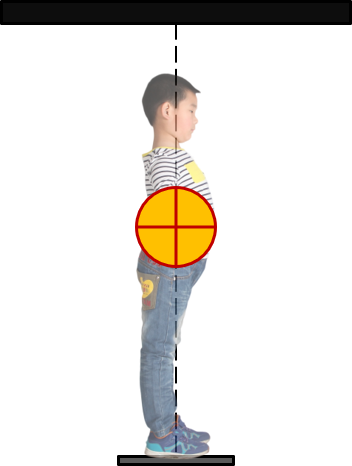
\includegraphics[]{images/child_vlp_standing.png}
      \caption{A person standing on a swing has their center of mass 
      close to the pivot.}
   \end{subfigure}
   \hfill
   \begin{subfigure}[t]{0.45\textwidth}
      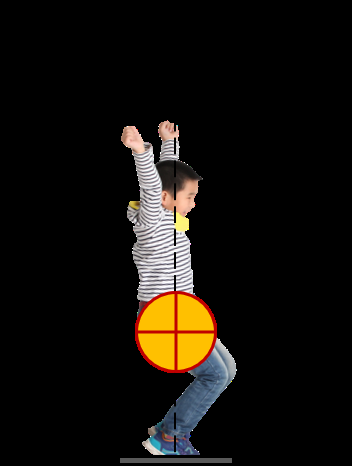
\includegraphics[]{images/child_vlp_squatting.png}
      \caption{When a person squats on a swing, their center of mass extends
      away from the pivot.}
   \end{subfigure}
   \caption{The VLP representation of a person on a standing swing.}
   \label{fig:child-vlp}
\end{figure}

The action of regulating pendulum length to inject energy into the VLP is known as
``pumping". \citet{pumping_swing_standing_squatting} asked whether
the pumping strategy performed by children is time-optimal, assuming the
children could squat or stand instantaneously. 
Indeed, they discovered that children increase the height of their swing as fast
as is physically possible.

A child's optimal pumping strategy is the following: 
they stand at the lowest point of the swing, and squat at the highest point.
Looking at the VLP representation, the pendulum shortens at the bottom of the
swing, and lengthens at the top. 
For an intuitive explanation, conservation of angular momentum indicates that
shortening the pendulum at the bottom forces the mass to gain speed to
compensate for the reduced length \cite{how_to_pump_a_swing}.
Energy is not conserved in this process, so the pendulum gains kinetic energy
and reaches a higher point at the peak of its swing.
Lengthening the pendulum when it reaches this peak means gravity
imparts a larger angular momentum to the mass by the time it reaches the bottom
of its swing, which in turn is converted to a higher velocity when the
pendulum is shortened.
By alternating these processes, the pendulum experiences an average net gain in
rotational energy.

Notice that the child's pumping strategy requires knowledge of
when the system is at the ``bottom" or ``top" of the swing. 
Since being at the bottom is equivalent to having angle \(q = 0\) and being
at the top is equivalent to having momentum \(p = 0\), a controller based on
this strategy will necessarily involve the full unactuated phase \((q,p)\). 
This is why we must use VNHCs instead of other methods (such as VHCs) 
to perform this maneuver.

The time-optimal controller from \cite{pumping_swing_standing_squatting} is, in
our notation,
\[
   L^\star(q,p) := -\sign{qp}
   ,
\]
which is a piecewise-continuous controller that varies between \(\pm 1\). 
We could set our constraint to be \(l = L^\star(q,p)\), but this is not a VNHC
because it is not \(C^2\).
Additionally, it would force us to assume that \(l \in \{-1,0,1\}\) and that one
can switch \(l\) instantaneously.
Since we need to enforce the constraint using the physical input \(\tau\) (which
would ideally emulate realistic human motion), we cannot use \(L^\star\) as our
VNHC.
We will instead find an alternate representation of \(L^\star\) which can be
converted into a VNHC, and which allows 
\(l \in [\underbar{l},\overbar{l}]\).

Figure \ref{fig:vlp-optimal-controller-qp-plane} displays \(L^\star(q,p)\) 
on the \((q,p)\)-plane.
Note that the length remains constant inside each quadrant and changes only when it
crosses one of the axes. Using this fact, we can redefine
the time-optimal pumping strategy as a function of 
\(\theta := \arctan_2(p,q)\).
Abusing notation, we denote this by \(L^\star(\theta)\), which is defined in
(\ref{eqn:vlp-optimal-controller}).
Figure \ref{fig:vlp-optimal-controller} shows the graph of \(L^\star(\theta)\), 
where now the length varies between \([\underbar{l},\overbar{l}]\) rather than 
\(\{-1,0,1\}\). 

\begin{equation}\label{eqn:vlp-optimal-controller}
   L^\star(\theta):= \begin{cases}
      \overline{l} & \theta \in [-\frac{\pi}{2},0[ \cup [\frac{\pi}{2}, \pi[ \\
      \underline{l} & \theta \in [-pi, -\frac{\pi}{2}[ \cup [0,\frac{\pi}{2}[ 
      .
   \end{cases}
\end{equation}

\begin{figure}
   \centering
   \begin{subfigure}[t]{0.45\textwidth}
      \includestandalone[width=\linewidth]{images/vlp_optimal_controller_qp_plane}
      \caption{The time-optimal controller \(L^\star(q,p)\) mapped onto the
      \((q,p)\)-plane. Here, red corresponds to \(L^\star(q,p) = -1\) and blue
      to \(L^\star(q,p) = 1\).}
      \label{fig:vlp-optimal-controller-qp-plane}
   \end{subfigure}
   \hfill
   \begin{subfigure}[t]{0.45\textwidth}
      \includestandalone[width=\linewidth]{images/vlp_optimal_controller}
      \caption{The time-optimal controller converted to the alternate
      representation \(L^\star(\theta)\).}
      \label{fig:vlp-optimal-controller}
   \end{subfigure}
   \caption{The time-optimal controller for a standing swing as derived by
      \cite{pumping_swing_standing_squatting}. The colour red
      corresponds to standing, blue to squatting, and 
      \(\theta := \arctan_2(p,q)\) is the angle of the VLP phase in the
      \((q,p)\)-plane.}
\end{figure}

We now define a continuous function which
approximates \(L^\star(\theta)\). 
Let \(\Delta l := (\overline{l} - \underline{l})/2\) and 
\(l_{\text{avg}} := (\overline{l} + \underline{l})/2\).
Let \(T \in \, ]0,\frac{\pi}{2}]\) be a parameter of our choosing.
By intelligently attaching sinusoids of frequency \(\omega = \frac{\pi}{T}\) to
\(L^\star(\theta)\) (see Figure \ref{fig:vlp-T-controller}), we get a family of
\(C^1\) constraints \(L_T(\theta)\) parameterized
by \(T\): 
\begin{equation}\label{eqn:vlp-T-controller}
   L_T(\theta) := \begin{cases}
      \overline{l} & \theta \in \left[-\frac{\pi}{2} + \frac{T}{2}, -\frac{T}{2}\right] 
      \cup \left[\frac{\pi}{2} + \frac{T}{2}, \pi - \frac{T}{2}\right] \\
      \underline{l} & \theta \in \left[-\pi + \frac{T}{2}, -\frac{\pi}{2} - \frac{T}{2}\right] 
      \cup \left[\frac{T}{2}, \frac{\pi}{2} - \frac{T}{2}\right] \\
      -\Delta l \sin(\omega(\theta + \pi)) + l_{\text{avg}} & \theta \in
      \left[-\pi,-\pi + \frac{T}{2}\right] \\
      -\Delta l \sin(\omega \theta) + l_\text{avg} & \theta \in [-\frac{T}{2},
      \frac{T}{2}] \\
      \Delta l \sin(\omega(\theta - a)) + l_\text{avg} & 
      \theta \in \left[a - \frac{T}{2}, a + \frac{T}{2}\right] \text{ for } 
      a \in \left\{-\frac{\pi}{2}, \frac{\pi}{2}\right\} \\
      -\Delta l \sin(\omega(\theta-\pi)) & \theta \in \left[\pi - \frac{T}{2},\pi\right] 
      .
   \end{cases}
\end{equation}

\begin{figure}
   \centering
   \includestandalone[width=0.7\textwidth]{images/vlp_T_controller}
   \caption{The continuous VLP constraint \(l = L_T(\theta)\).}
   \label{fig:vlp-T-controller}
\end{figure}

This family of constraints approximates \(L^\star(\theta)\) because 
\[
   \lim\limits_{T \rightarrow 0} L_T(\theta) = L^\star(\theta)
   .
\]
Unfortunately, while \(L_T(\theta)\) is continuously-differentiable, 
it is not twice-differentiable for most values of \(T\).
If we wish to use it as a VNHC, we must ensure that either the generalized
forces \(\tau\) acting on \(p_l\) can be discontinuous (which is certainly
achievable by humans), or we must find a value of \(T\) where this constraint is
at least \(C^2\).
Thankfully, setting \(T = \frac{\pi}{2}\) yields the smooth function 
\(L_{\frac{\pi}{2}}(\theta)\), which can be simplified from
(\ref{eqn:vlp-T-controller}) into
\begin{equation}\label{eqn:vlp-smoothed-controller}
   L_\frac{\pi}{2}(\theta) = -\Delta l \sin(2\theta) + l_{\text{avg}}
   .
\end{equation}
This smooth constraint is plotted for demonstration in Figure
\ref{fig:vlp-smoothed-controller}.

\begin{figure}
   \centering
   \includestandalone[width=0.6\textwidth]{images/vlp_smoothed_controller}
   \caption{The smoothed VLP constraint \(l = L_\frac{\pi}{2}(\theta)\).}
   \label{fig:vlp-smoothed-controller}
\end{figure}

Because \(L_\frac{\pi}{2}(\theta)\) is smooth and it approximates
\(L^\star(\theta)\), we set our VNHC to be
\[
   h(\mathbf{q},\mathbf{p}) = l - L_\frac{\pi}{2}\left(\theta(q,p)\right)
   .
\]

Before proving the VLP will gain energy under this VNHC, 
we must rigorously define what that means.
If any initial condition of the constrained dynamics converges to the point
\((q,p) = (0,0)\), the momentum must be decreasing over time, so the VLP will
clearly be losing energy.
A notion of energy injection must therefore require that the origin repels all
solutions.
We need to avoid closed orbits or limit cycles in the \((q,p)\)-plane,
so that the system can always reach higher speeds. 
Finally, we want the VLP's momentum to increase on average, regardless of
its initial value.
This intuition is captured mathematically by the following definition.

\begin{defn}\label{defn:energy-injection}
   Let \(D \subset \R^2\) with \(0 \in D\).
   Let \(f : D \rightarrow \R^2\) be locally Lipschitz with \(f(0) = 0\).
   The system described by \(\dot{x} = f(x)\) 
   \textit{gains energy on \(D\)} if 
   \begin{enumerate}
      \item The origin is a repeller 
         (or equivalently, the origin is asymptotically stable in negative time).
      \item For all compact sets \(K \subset D\) and for almost every initial
         condition \(x(0) \in K\), there exists \(T > 0\) such
         that \(x(t) \not \in K \, (\forall t > T)\).
   \end{enumerate}
   The system \textit{loses energy on \(D\)} if it gains energy in
   negative-time.
\end{defn}

The second property of Definition \ref{defn:energy-injection} allows the system
to have unstable equilibria, but not limit cycles nor closed orbits.
The next definition ties this notion of energy gain to VNHCs.

\begin{defn}
   A regular VNHC \(h(\mathbf{q},\mathbf{p}) = 0\) 
   \textit{injects (dissipates) energy} if the constrained dynamics gain (lose)
   energy everywhere on the constraint manifold, except possibly on a set of
   measure zero.
\end{defn}

We can now prove our VNHC injects energy into the VLP. 
As part of the proof, we will require the following lemma.

\begin{lemma}\label{lemma:sign-of-cube}
   For any \(x,y \in \R\),
   \[
      \sign{x^3 - y^3} = \sign{x-y}
      .
   \]
\end{lemma}
\begin{proof}
   Observe that \(x^3 - y^3 =  (x-y)(x^2 + xy + y^2)\).
   The inequality \(x^2 + xy + y^2 \geq 0\) holds because
   \[
      x^2 + xy + y^2 = \left(x  + \frac{y}{2}\right)^2 + \frac{3y^2}{4} \geq 0
      ,
   \]
   which proves the lemma.
\end{proof}

We will show that the constrained dynamics trace out a curve on the
\((q,p)\)-plane which is diverging from the origin.  
This implies that the momentum \(p\) is increasing in magnitude whenever the
curve hits the \(p\)-axis, which in turn means the VLP is gaining energy on
average.

\begin{thm}\label{thm:vlp-energy-stabilization}
   Define \(\theta := \arctan_2(p,q)\).
   Let \(L : \mathbb{S}^1 \rightarrow [\underline{l},\overline{l}]\) be a
   \(C^2\) function of \(\theta\).
   A regular VNHC of the form 
   \(h(\mathbf{q},\mathbf{p}) = l - L(\theta)\) injects energy into the VLP
   if there exists 
   \(l_\text{avg} \in [\underline{l},\overline{l}]\) such that 
   \begin{equation}\label{eqn:vlp-energy-gain-condition}
      \left(l_\text{avg} - L(\theta)\right)sin(2\theta) \geq 0 
      \text{ }\forall \theta \in \mathbb{S}^1
      ,
   \end{equation}
   with the property that the inequality is strict except at the
   coordinate axes.
   If the inequality is flipped, the VNHC dissipates energy. 
\end{thm}
\begin{proof}
   The constraint manifold for \(h\) is the cylinder \(\Gamma = \mathbb{S}^1 \times \R \). 
   In negative-time, the dynamics on \(\Gamma\) are
   \begin{equation}\label{eqn:negative-time-vlp}
      f(q,p) = 
      -\begin{bmatrix}
         \dot{q} \\ \dot{p}
      \end{bmatrix} = \begin{bmatrix}
         -\frac{p}{mL(\theta)^2} \\
         mgL(\theta)\sin(q)
      \end{bmatrix}
      .
   \end{equation}
   This has equilibria at \((q,p) = (0,0)\) and \((q,p) = (\pi,0)\) (the
   third ``equilibrium" \((-\pi,0)\) is the same as \((\pi,0)\) because 
   \(q \in \mathbb{S}^1\)).
   To prove the origin of the positive-time system (\ref{eqn:vlp-hamiltonian})
   is a repeller, we will show the origin of the negative-time system 
   (\ref{eqn:negative-time-vlp}) is almost everywhere globally asymptotically
   stable. 

   Choose, as a candidate Lyapunov function, the energy for the
   average-length pendulum with zero-potential at the bottom of the swing:
   \[
       E_\text{avg}(q,p) := \frac{1}{2}\frac{p^2}{m l_\text{avg}^2} 
           + m g l_\text{avg} (1-\cos(q))
      .
   \]
   This is positive definite at \((0,0)\) and has compact sublevel
   sets on \(\Gamma\). 
   The derivative of \(E_\text{avg}\) along (\ref{eqn:negative-time-vlp}) is
   \[
      \dot{E}_\text{avg} = \frac{g\sin(q)p \left(L(\theta)^3 - l_\text{avg}^3\right)}
              {l_\text{avg}^2L(\theta)^2}
      .
   \]
   The sign of \(\sin(q)p\) depends only on the quadrant in the
   \((q,p)\)-plane. In fact, it is easy to show that
   \[
      \sign{\sin(q)p} = \sign{\sin(2\theta)}
      .
   \]
   Furthermore, by Lemma \ref{lemma:sign-of-cube} we have
   \[ 
       \sign{L(\theta)^3 - l_\text{avg}^3} = \sign{L(\theta) - l_\text{avg}}
       .
   \]
   The derivative of \(E_\text{avg}\) is never positive since
   \begin{align}\label{eqn:vlp-proof-neg-inv}
    \sign{\dot{E}_\text{avg}} &= \sign{\sin(q)p \left(L(\theta)^3 - l_\text{avg}^3\right)}
          \nonumber \\
          &= \sign{\sin(2\theta) \left(L(\theta) - l_\text{avg}\right)}
          \nonumber \\
          &= -\sign{(l_\text{avg} - L(\theta))\sin(2\theta)} 
          \nonumber \\
          &\leq 0 \text{ (by assumption)}
      .
   \end{align}
   Thus, \(E_\text{avg}\) is a Lyapunov function, which means the negative-time system is
   stable \cite{lyapunov}. 

   The linearization of (\ref{eqn:negative-time-vlp}) at the upright equilibrium
   \((\pi, 0)\) is given by
   \[
      df_{(\pi,0)} = \begin{bmatrix}
         0 & -\frac{1}{mL(0)^2} \\
         -m g L(0) & 0 \\
      \end{bmatrix}
      ,
   \]
   which has eigenvalues at \(\lambda = \pm \sqrt{\frac{g}{L(0)}}\).
   The positive-time system (\ref{eqn:vlp-hamiltonian}) has the same eigenvalues
   at this equilibrium.
   Label the set of initial conditions converging to \((\pi, 0)\) in
   positive time by
   \[
      \Pi_0^+ := \left\{ (q_0,p_0) \in \Gamma \mid \lim_{t \to \infty} (q(t),p(t)) = (\pi, 0) \right\}
      ,
   \]
   and the set of initial conditions converging to \((\pi,0)\)
   in negative time by \(\Pi_0^-\).
   Since only one eigenvalue is negative, the stable manifold theorem tells us
   that both \(\Pi_0^+\) and \(\Pi_0^-\) are one-dimensional.
   While this implies the origin is not globally asymptotically stable for
   (\ref{eqn:negative-time-vlp}), we can still show it is asymptotically stable
   for almost every initial condition because \(\Pi_0^+\) and \(\Pi_0^-\) are of
   measure zero within \(\Gamma\).

   Define \(D := \Gamma \backslash \Pi_0^-\) to be the domain of interest.
   Using a Krasovskii-LaSalle argument \cite{krasovskii_lasalle}, 
   we will prove that (\ref{eqn:negative-time-vlp}) asymptotically converges to
   \((0,0)\) if it is initialized on \(D\).
   First, we define the zero-set
   \[
      Z = \left\{(q,p) \in \Gamma \mid 
      \dot{E}_\text{avg}(q,p) = 0 \right\}
      .
   \]
   It is easy to show that \(Z\) is the union of the coordinate axes
   \[
      Z= \mathbb{S}^1 \times \left\{0\right\} \cup 
         \left\{0\right\} \times \R
      .
   \]
   Krasovskii-LaSalle tells us that solutions to (\ref{eqn:negative-time-vlp})
   converge to the largest invariant set in \(Z \cap D\).
   Since \(f(q,p) = (0,0)\) on \(D\) only when \((q,p) = (0,0)\),
   the origin is asymptotically stable on \(D\) for the negative-time system.
   Hence, the positive-time system is diverging away from the origin 
   in the \((q,p)\) plane, which means the origin is a repeller.

   We now prove the system escapes compact sets in finite time.
   Let \(x(t) = (q(t),p(t))\) be the orbit for the positive-time system.
   Let \(K \subset \Gamma\) be compact and assume \(x(0) \in K\backslash \Pi_0^+\).
   For a proof by contradiction, suppose that for all \(T > 0\) there exists
   \(t' > T\) where \(x(t') \in K\).
   Let 
   \[
      k := \max\limits_{(q,p) \in K} E_\text{avg}(q,p)
      ,
   \] 
   be the largest energy value attained in \(K\), and let its sublevel set be
   \[
      E_k := \left\{ (q,p) \in \Gamma \mid E_\text{avg}(q,p) \leq k \right\}
      .
   \]
   All sublevel sets of \(E_\text{avg}\) are compact, negatively
   invariant (by (\ref{eqn:vlp-proof-neg-inv})), and \(E_k\) contains \(K\).
   We assumed \(x(t') \in K\), so it follows that \(x(t') \in E_k\). 
   Then, since \(E_k\) is negatively invariant, the half orbit
   \(x([0,t'])\) is contained fully within \(E_k\).
   In particular, \(x(T) \in E_k\);
   but \(T\) was chosen arbitrarily, which implies \(x(t) \in E_k\) for all
   \(t \in [0,\infty[\).
   Since \(E_k\) is compact, \(x(t)\) has a positive limit set in
   \(E_k\) which (by Poincar\'{e}-Bendixson) is either an equilibrium or a
   closed orbit \textbf{SOURCE?}.
   The system cannot have closed orbits, since this would violate asymptotic
   stability of \((0,0)\) in negative time. 
   Hence, the positive limit set must be one of the equilibria. 
   The origin is a repeller, which means \(x(t)\) must be converging to 
   \((\pi,0)\).
   This is a contradiction, since we assumed \(x(0) \not \in \Pi_0^+\).

   We have shown that orbits of the constrained dynamics will leave compact sets in
   finite time, including all sublevel sets of \(E_\text{avg}\). 
   The orbit \((q(t),p(t))\) is spiraling away from the origin and, for almost
   all initial conditions, will not converge to the upper equilibrium.
   Thus, the VLP is gaining energy on average because its momentum is increasing.
   Flipping the inequality of (\ref{eqn:vlp-energy-gain-condition}) 
   means \(E_\text{avg}\) is a Lyapunov function for the positive time system;
   by the same arguments presented here, the VLP loses energy while
   converging asymptotically to \((0,0)\).
 \end{proof}

\begin{cor}
   Recall that
   \[
      L_\frac{\pi}{2}(\theta) := -\Delta l \sin(2\theta) + l_\text{avg}
      ,
   \]
   and define 
   \[
      L^{-}_\frac{\pi}{2}(\theta) := \Delta l \sin(2\theta) + l_\text{avg}
      .
   \]
   The VNHC \(l = L_\frac{\pi}{2}(\theta)\) injects energy into the VLP,
   while \(l = L^{-}_\frac{\pi}{2}(\theta)\) dissipates energy.
\end{cor}
\begin{proof}
   Both VNHCs satisfy Theorem \ref{thm:vlp-energy-stabilization} because
   \[
      \left(l_\text{avg} - L_\frac{\pi}{2}(\theta)\right)\sin(2\theta) = 
      \Delta l \sin^2(2\theta) \geq 0
      ,
   \] 
   and
   \[
      \left(l_\text{avg} - L^{-}_\frac{\pi}{2}(\theta)\right)\sin(2\theta) = 
      - \Delta l \sin^2(2\theta) \leq 0
      ,
   \] 
   where the inequalities are strict everywhere except the coordinate axes.
\end{proof}


The class of VNHCs which satisfies Theorem \ref{thm:vlp-energy-stabilization} is
illustrated graphically in Figure \ref{fig:vlp-energy-in-out}. 
To stabilize specific energy level sets, one simple approach is to switch
between injection and dissipation VNHCs when the momentum \(p\) reaches
a pre-determined value at the bottom of the swing.
For the VNHCs we designed in this chapter, this means toggling
between \(L_\frac{\pi}{2}(\theta)\) and \(L^{-}_\frac{\pi}{2}(\theta)\),
with some hysteresis to avoid infinite switching.  

\begin{figure}
   \centering
   \includestandalone[width=0.5\textwidth]{images/vlp_energy_in_out}
   \caption{Any VNHC of the form \(l = L(\theta)\) where \(L(\theta)\)
      is entirely contained within
      the green (yellow) regions will inject (dissipate) energy.}
      \label{fig:vlp-energy-in-out}
\end{figure}

Theorem \ref{thm:vlp-energy-stabilization} provides an alternate
explanation for why the optimal pumping strategy \(L^\star(\theta)\) works
so well at injecting energy: it maximizes the derivative of \(E_\text{avg}\)
under the restriction \(l \in [\underline{l},\overline{l}]\), so that the orbit
in the \((q,p)\)-plane diverges from the origin as fast as possible. 

Let us define \((L^\star)^{-}(\theta)\) by swapping the order of 
\(\underline{l}\) and \(\overline{l}\) in \(L^\star(\theta)\): 
\[
   (L^\star)^-(\theta) := \begin{cases}
      \underline{l} & \theta \in [-\frac{\pi}{2},0[ \cup [\frac{\pi}{2}, \pi[ \\
      \overline{l} & \theta \in [-pi, -\frac{\pi}{2}[ \cup [0,\frac{\pi}{2}[ 
      .
   \end{cases}
\]
Since this function \textit{minimizes} the derivative of \(E_\text{avg}\) under
the restriction \(l \in [\underline{l},\overline{l}]\), one might predict that 
\((L^\star)^{-}(\theta)\) is the optimal energy dissipation strategy for the VLP.
This is, in fact, true. \citet{pumping_swing_standing_squatting} showed 
that squatting at the lowest point of a swing and standing at the highest
(instead of standing and squatting, respectively) produces the
time-optimal trajectory for \textit{stopping} a standing swing. 

All together, the theory developed in this chapter shows that VNHCs can
replicate the time-optimal pumping/dissipation strategies performed by humans on
swings.
Furthermore, we see that VNHCs are a powerful tool for creating simple energy
stabilization techniques based on natural human motion.

\section{Simulation Results}
% TODO: Show the simulations of the VLP VNHCs (multiple of them). How does the
% energy injection time of our sin(2theta) VNHC compare to the energy injection
% time of the optimal one? How does the VNHC version compare in robustness with
% the time-based one from the pumping paper?

%/========== /Variable Length Pendulum ==========/%
% vim: set ts=3 sw=3 sts=0 et tw=80 ffs=unix :
